\documentclass[xcolor=table,10pt,final]{beamer}
\renewcommand\mathfamilydefault{\rmdefault}

\setbeamertemplate{navigation symbols}{}
\usepackage{amsmath,amsfonts,amssymb,pxfonts,xspace}
\usepackage{textcomp}
\usepackage{lmodern}
\usepackage{verbatim}
\usepackage{graphicx}
\usepackage{listings}
\usepackage[T1]{fontenc}

\lstset{
    basicstyle=\footnotesize,
    keywordstyle=\color[rgb]{0.1,0.8,0.1}\bfseries,
    commentstyle=\color{blue},
    numbers=left,
    stringstyle=\ttfamily\color{red!50!brown},
    showstringspaces=false}
\lstset{literate=%
   *{0}{{{\color{red!20!violet}0}}}1
    {1}{{{\color{red!20!violet}1}}}1
    {2}{{{\color{red!20!violet}2}}}1
    {3}{{{\color{red!20!violet}3}}}1
    {4}{{{\color{red!20!violet}4}}}1
    {5}{{{\color{red!20!violet}5}}}1
    {6}{{{\color{red!20!violet}6}}}1
    {7}{{{\color{red!20!violet}7}}}1
    {8}{{{\color{red!20!violet}8}}}1
    {9}{{{\color{red!20!violet}9}}}1
}



\begin{document}

\title{Python for Scientific Computing}
\subtitle{Lecture 1: The Python Calculator}
\author{Albert DeFusco\\Center for Simulation and Modeling}
\date{\today}
\frame{\titlepage}

\begin{frame}
  \frametitle{Computer programming}
    assembly
\end{frame}
\begin{frame}
  \frametitle{Computer programming}
compiled code
\end{frame}
\begin{frame}
  \frametitle{Computer programming}
  interpreted code
\end{frame}

\begin{frame}
  \frametitle{What's so great about Python?}
  \begin{itemize}
    \item portable
      \begin{itemize}
        \item not the programmer's responsibility
      \end{itemize}
  \end{itemize}
\end{frame}
\begin{frame}
  \frametitle{What's so great about Python?}
  \begin{itemize}
    \item efficient
      \begin{itemize}
        \item rich features built in
        \item clean syntax
        \item focus shifts to ``algorithm'' and away from implementation
      \end{itemize}
  \end{itemize}
\end{frame}
\begin{frame}
  \frametitle{What's so great about Python?}
  \begin{itemize}
    \item extendible
      \begin{itemize}
        \item Plenty of easy-to-use modules
        \item Use C or Fortran routines directly
          \begin{itemize}
            \item separate interface from implementation
          \end{itemize}
      \end{itemize}
    \item A whole Python program can
      \begin{enumerate}
        \item read data
        \item do computation
        \item visualize results
      \end{enumerate}
  \end{itemize}
\end{frame}

\begin{frame}[fragile]
  \frametitle{Why use python for science?}
  \begin{itemize}
    \item a highly programmable a calculator
    \item fast proto-typing a new algorithm or program design
    \item many science and mathematics modules already exist
  \end{itemize}
\end{frame}

\begin{frame}
  \frametitle{Development Environment}
  \begin{columns}
    \begin{column}{0.5\paperwidth}
      \begin{itemize}
        \item Frank
      \end{itemize}
    \end{column}
    \begin{column}{0.5\paperwidth}
      \centering
      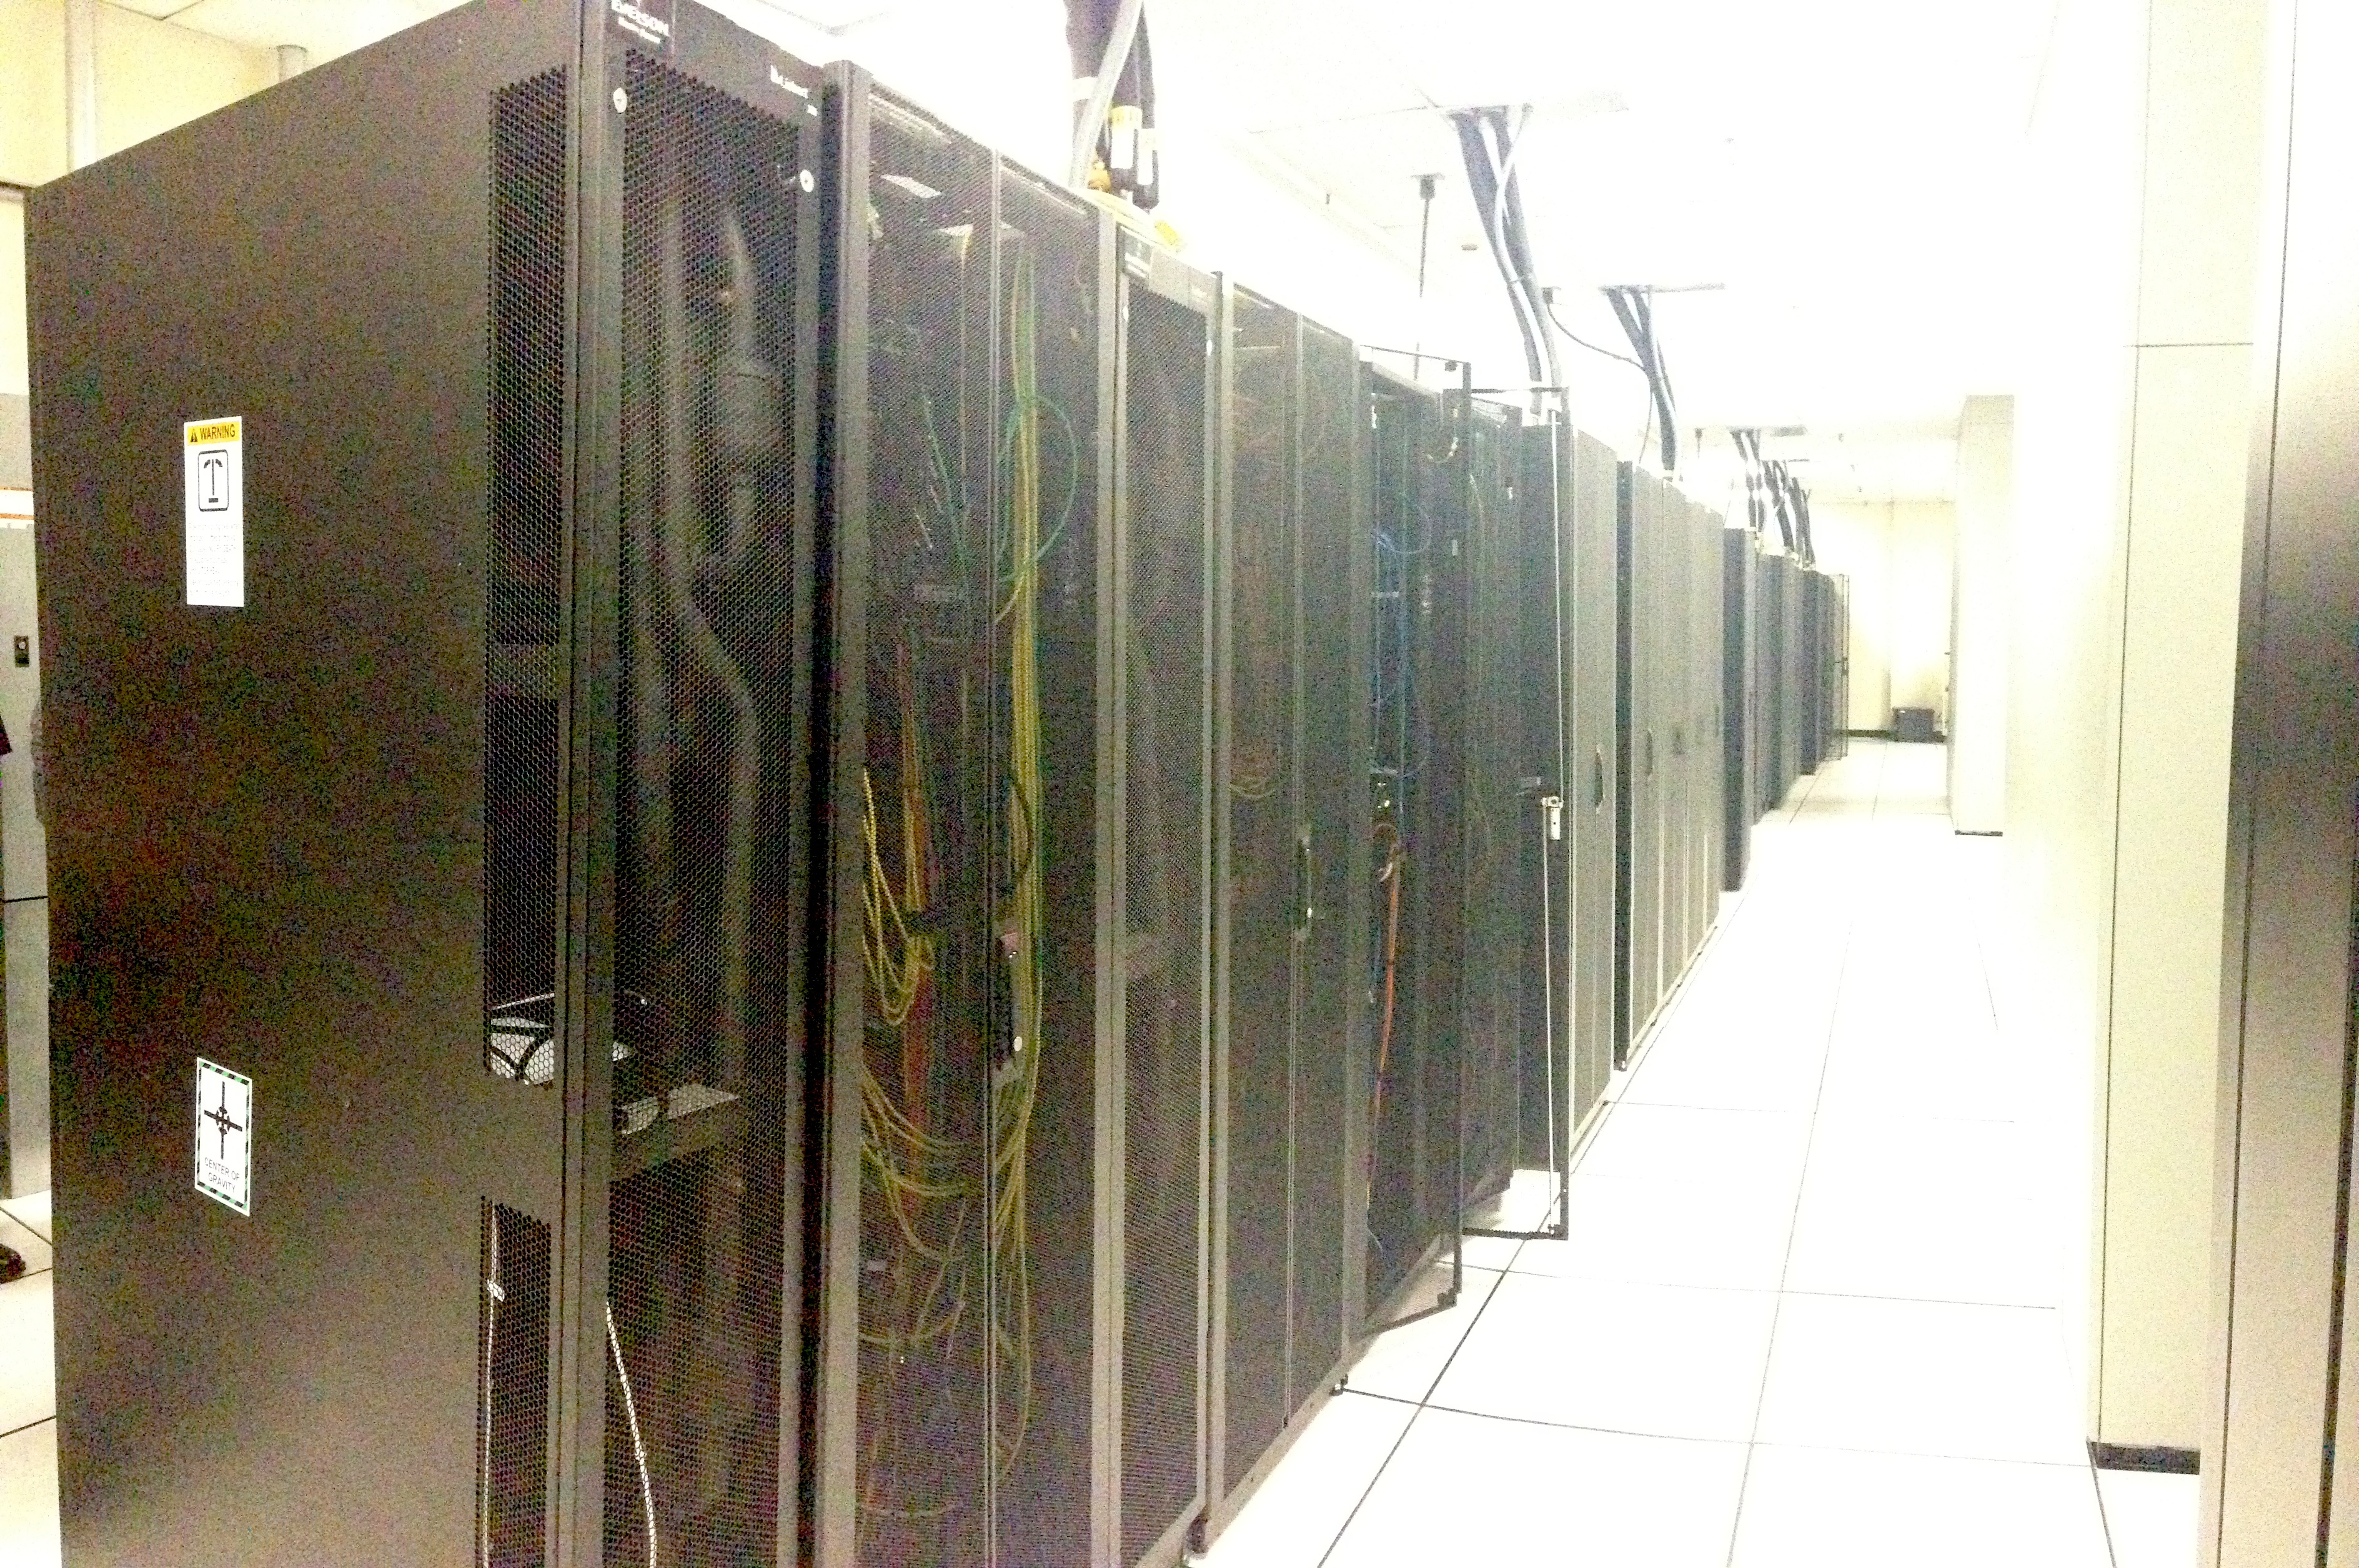
\includegraphics[width=0.48\paperwidth]{figures/frank}
    \end{column}
  \end{columns}
\end{frame}

\begin{frame}[fragile]
  \frametitle{Read the documentation}
  \begin{verbatim}
> pydoc

> python
>>> help()
\end{verbatim}
\end{frame}




\begin{frame}[fragile]
  \frametitle{Disclaimer}
  Python 2.7 $!=$ 3.0
  \vskip1cm
  \begin{verbatim}
http://wiki.python.org/moin/Python2orPython3
\end{verbatim}
\end{frame}

\begin{frame}
  \frametitle{Python syntax}
  \begin{itemize}
    \item Extremely simplified syntax
      \begin{itemize}
        \item nearly devoid of special characters
      \end{itemize}
    \item Implicit types
      \begin{itemize}
        \item It is the responsibility of the programmer
        \item Types can change
      \end{itemize}
  \end{itemize}
\end{frame}

\begin{frame}[fragile]
  \frametitle{Python objects}
  \begin{itemize}
    \item All data in Python is represented by objects
    \item Objects have
      \begin{itemize}
        \item an identity
        \item a type
        \item a value
        \item a name (``variable'')
      \end{itemize}
    \item Variables are names assigned to {\tt objects}
  \end{itemize}
\end{frame}

\begin{frame}[fragile]
  \frametitle{Numerical objects}
  \begin{itemize}
    \item Integers
      \begin{itemize}
        \item \lstinline[language=python]|a = 1|
      \end{itemize}
    \item Floats
      \begin{itemize}
        \item \lstinline[language=python]|a = 1.0|
        %\item {\tt numpy} provides precision control
      \end{itemize}
    \item Complex numbers
      \begin{itemize}
        \item \lstinline[language=python]|a = 1.5 + 0.5j|
        \item \lstinline[language=python]|a.real| and \lstinline[language=python]|a.imag| return each component
      \end{itemize}
    \item Type casts
      \begin{itemize}
        \item \lstinline[language=python]|myFloat = float(myInteger)|
        \item \lstinline[language=python]|myInt = int(myFloat)|
      \end{itemize}
    \item Operators
      \begin{itemize}
        \item Addition \lstinline[language=python]|+|
        \item Subtraction \lstinline[language=python]|-|
        \item Multiplication \lstinline[language=python]|*|
        \item Exponentiation \lstinline[language=python]|**|
        \item Division \lstinline[language=python]|/|
        \item Modulus \lstinline[language=python]|%|
      \end{itemize}
  \end{itemize}
\end{frame}

\begin{frame}
  \frametitle{Logicals}
  \begin{itemize}
    \item Boolean type
      \begin{itemize}
        \item \lstinline[language=python]|a = (3 > 4)|
      \end{itemize}
    \item Comparisons
      \begin{itemize}
        \item \lstinline[language=python]|==|
        \item \lstinline[language=python]|!=,<>|
        \item \lstinline[language=python]|>|
        \item \lstinline[language=python]|<|
        \item \lstinline[language=python]|<=|
        \item \lstinline[language=python]|>=|
      \end{itemize}
  \end{itemize}
\end{frame}

\begin{frame}
  \frametitle{Logical operations}
  \begin{itemize}
    \item \lstinline[language=python]|not|, \lstinline[language=python]|and|, \lstinline[language=python]|or|
  \end{itemize}
\end{frame}

\begin{frame}[fragile]
  \frametitle{Strings}
  \begin{itemize}
    \item \lstinline[language=python]|a = 'single quoted'|
    \item \lstinline[language=python]|a = "double quoted"|
    \item Triple quotes preserve whitespace and newlines
  \end{itemize}
      \begin{lstlisting}[language=python]
      a = """triple
      quoted
      string"""
      \end{lstlisting}
      \begin{itemize}
    \item ``\symbol{92}'' is the escape character
  \end{itemize}
\end{frame}

\begin{frame}
  \frametitle{String operations}
  \begin{itemize}
    \item \lstinline[language=python]|doubleA = float(a)|
    \item \lstinline[language=python]|intA = int(a)|
    \item \lstinline[language=python]|wordList = a.split()|
  \end{itemize}
\end{frame}

\begin{frame}[fragile]
  \frametitle{Formatted strings}
  \begin{itemize}
    \item printing with placeholders
      \begin{table}
        \begin{tabular}{cl}
          \lstinline[language=python]|\%s| & string\\
          \lstinline[language=python]|\%d| & integer\\
          \lstinline[language=python]|\%f| & float with 6 decimals\\
          \lstinline[language=python]|\%E| & scientific notation\\
          \lstinline[language=python]|\%\%| & the \% sign
        \end{tabular}
      \end{table}
    \item modifiers
      \begin{itemize}
        \item integers after \% adjust with width to print
        \item decimal points are specified after the width as ``.x''
        \item use a hyphen after \% to left justify
        \item printing long strings or large numbers will skew columns
      \end{itemize}
  \end{itemize}
\begin{lstlisting}[langage=python]
v0=5
g=9.81
t=0.6
y=v0*t - 0.5*g*t**2
print """
At t=%f s, a ball with
initial velocity v0=%.3E m/s
is located at the height of %.2f m.
""" % (t, v0, y)
\end{lstlisting}
\end{frame}

\begin{frame}
  \frametitle{Printing information}
  \begin{itemize}
    \item print anything using \lstinline[language=python]|print|
    \item separate objects with \lstinline[language=python]|,|
    \item newline: \lstinline[language=python]|\\n|
  \end{itemize}
\end{frame}

\begin{frame}
  \frametitle{Structured blocks}
  \begin{itemize}
    \item {\tt if}, {\tt for}, {\tt while}
  \end{itemize}
\begin{lstlisting}
if (a>b):
  print 'a is bigger'
else if (b>a):
  print 'big is bigger'
else
  print 'a must equal b'
\end{lstlisting}
\end{frame}

\begin{frame}[fragile]
  \frametitle{Simple loops}
  \begin{itemize}
    \item \lstinline[language=python]|range(start,stop,step)|
      \begin{itemize}
        \item list of integers from start to stop-1 in step increments
        \item End point is always omitted
      \end{itemize}
  \end{itemize}
\begin{lstlisting}
for i in range(4):
  print i
-----------------
0
1
2
3
\end{lstlisting}
\end{frame}

\begin{frame}
  \frametitle{Mathematical Exercise 2}
  Compute a table of temperature conversion
  \vskip1cm
  \begin{equation*}
    C = \frac{5}{9}\left(F - 32\right)
  \end{equation*}
\end{frame}

\begin{frame}
  \frametitle{Mathematical Exercise 1}
  Compute Pi using the Wallis formula
  \vskip1cm
  \begin{equation*}
    \pi = 2\prod^{\infty}_{i=1}\frac{4i^2}{4i^2-1}
  \end{equation*}
\end{frame}


\end{document}
